\begin{exercise}
  Gesucht ist die Lösung $u$ des Poisson Problems
  \begin{align}\label{one}
    -\partial_x (k(x)\partial_x u(x))
    =
    \cos(x),
    \quad
    x \in (0,2\pi)
  \end{align}

  mit $u(0) = u(2\pi) = 1$ und gegebenen Wärmeleitkoeffizienten $k$. Sie
  beschreibt die Temperaturverteilung in einem dünnen Stab.

  \begin{itemize}
  \item[a)] Lösen Sie das Problem exakt bei konstanten $k(x) = k_0$ für alle
  $x \in [0, 2\pi]$.

  \item[b)] Lösen Sie das gleiche Problem numerisch mit Hilfe des Finite-Differenzen
  Verfahrens und untersuchen Sie für unterschiedliche $h$ die Größe des Fehlers.

  \item[c)] Wie könnte man \eqref{one} interpretieren, wenn der Wärmeleitkoeffizient
  nur stückweise konstant ist, d.h. wenn z.B. $k(x) = k_1$ für $x \in [0, \pi)$ und
  $k(x) = k_2 \neq k_1$ für $x \in (\pi, 2\pi]$? Berechnen Sie wiederum die analytische
  Lösung und schlagen Sie ein geeignetes Diskretisiertungsverfahren vor.
  \end{itemize}
\end{exercise}

\begin{solution}\leavevmode \\
  \begin{itemize}
    \item[a)] Bei konstantem $k_0$ vereinfacht sich unsere Differentialgleichung zu

    \begin{align*}
      -k_0 u ^\primeprime(x) = \cos(x).
    \end{align*}

    Durch zweimaliges Integrieren erhalten wir für unsere Lösung die Form

    \begin{align*}
      u(x)
      =
      \frac{1}{k_0}(\cos(x)+ax+b)
    \end{align*}

    mit (noch) unbekannten $a,b \in \R$. Um diese zu bestimmen sehen wir uns die
    Randwerte an. Bei $x=0$ erhalten wir:

    \begin{align*}
      u(0)
      = \frac{1}{k_0}(\cos(0)+0a+b) =
      \frac{1}{k_0}(1+b)
      \stackrel{!}{=}
      1
    \end{align*}

    womit wir $b = k_0 -1$ erhalten. Durch die zweite Randbedingung erhält man

    \begin{align*}
      u(2\pi) = \frac{1}{k_0}(\cos(2\pi) + ax + k_0 - 1) =
      \frac{1}{k_0}(ax + k_0) \stackrel{!}{=} 1,
    \end{align*}
    dass $a = 0$ und somit unsere analytische Lösung
    \begin{align*}
      u(x)
      =
      \frac{1}{k_0}(\cos(x)+k_0-1).
    \end{align*}
    \FloatBarrier
    \item[b)] Siehe Code.
    \includegraphicsboxed{example7.8.png}
    \begin{figure}
        \centering
        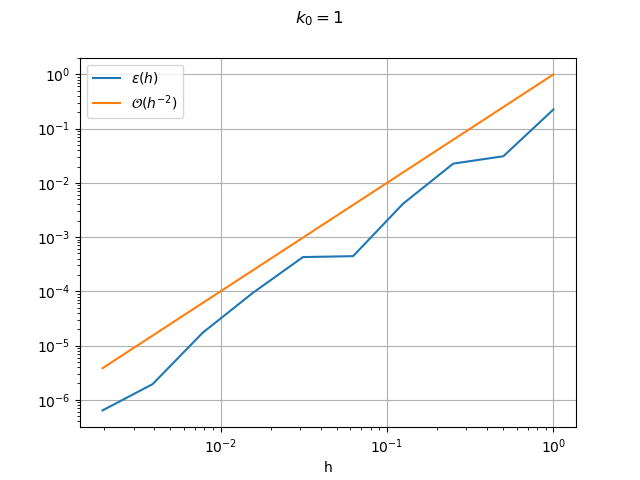
\includegraphics[width=\linewidth]{plot57.png}
    \end{figure}

    \item[c)] Bei stückweise konstanten Wärmeleitkoeffizienten haben wir eine
    Fallunterscheidung vorzunehmen. Man könnte \eqref{one} physikalisch so sehen,
    dass der Stab aus zwei verschiedenen Materialien besteht.

    Unsere Differentialgleichung lautet nun

    \begin{align*}
      u^\primeprime(x)
      =
      \begin{cases}
        -\frac{1}{k_1} \cos(x), & x \in [0,\pi) \\
        -\frac{1}{k_2} \cos(x), & x \in (\pi, 2\pi]
      \end{cases}
    \end{align*}

    Wieder integrieren wir und erhalten

    \begin{align*}
      u(x)
      =
      \begin{cases}
        \frac{1}{k_1}(\cos(x) + c_{00}x + c_{01}), & x \in [0,\pi) \\
        \frac{1}{k_2}(\cos(x) + c_{10}x + c_{11}), & x \in (\pi, 2\pi]
      \end{cases}
    \end{align*}

    Um $c_{00}, c_{10}, c_{01}, c_{11} \in \R$ zu bestimmen haben wir die zwei
    Randwertbedingungen. Zusätzlich soll ja auch $u \in C^1([0,2\pi])$ sein. Wir
    bekommen also noch zwei weitere Gleichungen.

    Aus $u(0)= 1$ erhalten wir, wie schon beim ersten Unterpunkt, $c_{01} = k_1-1$. \\
    Wegen der Stetigkeit im Punkt $\pi$ erhalten wir:

    \begin{align*}
      \frac{1}{k_1}(\cos(\pi) + c_{00}\pi + c_{01})
      &=
      \lim_{x \rightarrow \pi^-} u(x)
      \stackrel{!}{=}
      \lim_{x \rightarrow \pi^+} u(x)
      =
      \frac{1}{k_2}(\cos(\pi)+ c_{10}\pi + c_{11}) \\
      &\Rightarrow
      2k_2 -k_1 k_2 -k_1 = c_{00}\pi k_2 - c_{10}\pi k_1 - c_{11} k_1
    \end{align*}

    Aus der stetigen Differenzierbarkeit:

    \begin{align*}
        \frac{1}{k_1}(-\sin(\pi) + c_{00})
        &=
        \lim_{x \rightarrow \pi^+} u^\prime(x)
        \stackrel{!}{=}
        \lim_{x \rightarrow \pi^-} u^\prime(x)
        =
        \frac{1}{k_2}(-\sin(\pi)+ c_{10}) \\
        \Rightarrow
        k_2 c_{00}- k_1 c_{10} = 0
    \end{align*}

    Aus der rechten Randbedingung erhalten wir:

    \begin{align*}
      u(2\pi)
      =
      \frac{1}{k_2}(1 + c_{10}2\pi + c_{11})
      \stackrel{!}{=}
      1 \\
      \Rightarrow
      c_{10}2\pi +c_{11} = k_2 - 1
    \end{align*}

    Nun können wir ein lineares Gleichungssystem aufstellen um die restlichen
    Werte zu bestimmen:

    \begin{align*}
      \left( \begin{array}{ccc}
        \pi k_2 & -\pi k_1 & - k_1 \\
        k_2 & -k1 & 0 \\
        0 & 2\pi & 1
      \end{array}
      \right) \left(
      \begin{array}{c}
        c_{00} \\
        c_{10} \\
        c_{11}
      \end{array}
      \right)
      =
      \left(
      \begin{array}{c}
      2k_2 - k_1 k_2 - k_1 \\
      0 \\
      k_2 - 1
      \end{array}
      \right)
    \end{align*}
    Die Matrix ist dabei für $k_1k_2 \neq 0$ regulär, da für die Determinante gilt
    \begin{align*}
      \det(A) = -k_1k_2\pi -2k_1k_2\pi + k_1k_2\pi = -2k_1k_2\pi.
    \end{align*}
    Wir erhalten (mit Sympy) den Lösungsvektor
    $(\frac{k_2 - k_1}{k_2\pi}, \frac{k_2 - k_1}{k_1\pi}, k_2 + 1 - \frac{2k_2}{k_1})^{\top}$.
    Für ein geeignetes Diskretisiertungsverfahren muss man nun unterscheiden, ob
    $N$ gerade oder ungerade ist. Falls $N$ ungerade ist können wir die Diskretisierung
    wie im Skrip durchführen, dann gilt somit

    \begin{align*}
      -\frac{k_1}{h^2} y_2 + \frac{2k_1}{h^2} y_1
      =
      \cos(x_1) + \frac{k_1}{h^2}
      \quad
      & j = 1 \\
      -\frac{k_1}{h^2} y_{j-1} + \frac{2k_1}{h^2} y_j - \frac{k_1}{h^2}y_{j+1}
      =
      \cos(x_j)
      \quad
      &j \in \{2, \dots, \frac{N}{2}-1\} \\
      -\frac{k_2}{h^2} y_{j-1} + \frac{2k_2}{h^2} y_j - \frac{k_2}{h^2}y_{j+1}
      =
      \cos(x_j)
      \quad
      &j \in \{\frac{N}{2}+1, \dots , N-2\} \\
      -\frac{k_2}{h^2} y_{N-1} + \frac{2k_1}{h^2} y_{N-2}
      =
      \cos(x_{N-1})+ \frac{k_2}{h^2}
      \quad
      & j = N-1
    \end{align*}

    Für den Fall, dass $N$ gerade ist muss man $x_j = \pi$ gesondert behandeln, dort
    könnte man z.B. $k_3 = \frac{k_1 +k_2}{2}$ einführen und an diesem Punkt die Gleichung

    \begin{align*}
    -\frac{k_3}{h^2} y_{j-1} + \frac{2k_3}{h^2} y_j - \frac{k_3}{h^2}y_{j+1}
    =
    \cos(x_j)
    \end{align*}

    verwenden.
  \end{itemize}
\end{solution}
